\section{Centralized Authority}

A common way to implement auditability in private systems is to introduce a centralized authority or group of authorities (multi-party computation). Such authority can either be an external designated auditor or can enforce the internal policy rules in each transaction (accountability). 

According to this approach users embed auxiliary information to the transactions that are encrypted under the public key of a designated trusted auditor (\autoref{fig:cent-aud}). Therefore, the users data are remain private for the rest of the system's participants except the centralized authority, which can decrypt the auxiliary information at any point without the consent of the users. 

\begin{figure}
    \centering
    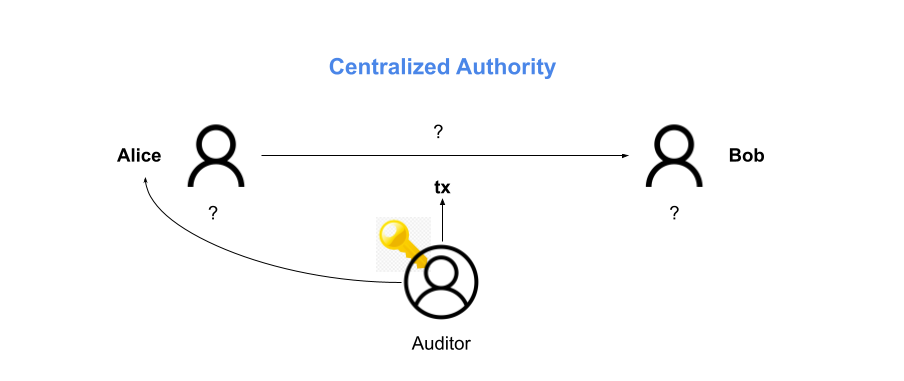
\includegraphics[width=0.9\textwidth]{images/privacy/Auditability in blockchain - Centralized.png}
    \caption{Auditability - Centralized Authority}
    \label{fig:cent-aud}
\end{figure}


This method can be a trivial solution for adding auditability to privacy-preserving systems. However, all the data is collected by a single centralized authority, which accumulates excessive power. This fact can negatively impact the user privacy.

One example that implement this approach is presented below:

\subsection{Zcash extension}
% \subsection{PRCash}
% \subsection{ACCDET}


\section{General Auditor}

In order to avoid gathering all the information to one (or a group) centralized authority a second approach were proposed. That is an interactive protocol between the user being audited and the auditor. In this case, the auditor, who can be \textit{any} auditing authority, can ask specified questions which derives from system's policies. Users answer to this questions with zero-knowledge proofs based on data that are stored on chain (\autoref{fig:gen-aud}).

This protocol implies the concent and the cooperation from the audited user. However, this requirement cannot be exploited by non-compliant users due to the fact that refusal to cooperate with authorities can be considered equivalent to a failed audit.

\begin{figure}
    \centering
    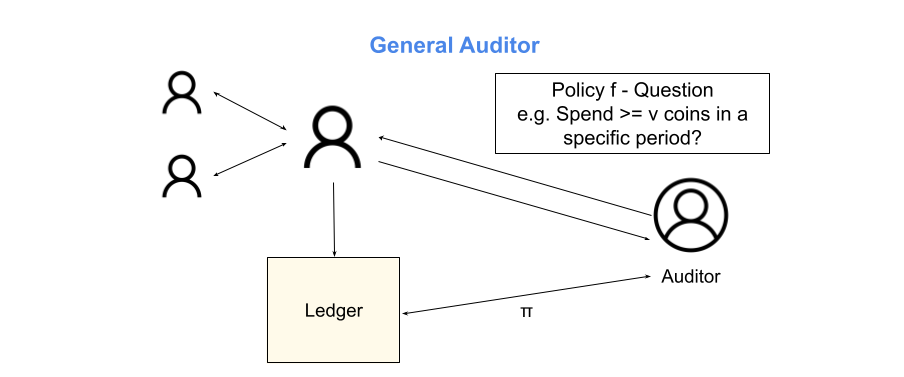
\includegraphics[width=0.9\textwidth]{images/privacy/Auditability in blockchain - General Auditor.png}
    \caption{Auditability - General Auditor}
    \label{fig:gen-aud}
\end{figure}

Some typical examples of auditable private decentralized systems who implement a general auditor are presented below:

\subsection{zkLedger}
% \subsection{miniLedger}
\subsection{PGC}